\documentclass[../../main.tex]{subfiles}

% 

\begin{document}
\chapter{Spektroskopie záření beta a elektronová spektroskopie}

\section{Interakce lehkých nabitých částic s hmotou}

Lehké nabité částice na rozdíl od těžkých nabitých částic ztrácejí svoji energii na mnohem kratších vzdálenostech ($10^{-3} ~\mathrm{m}$) a mají daleko klikatější trajektorii materiálem absorbátoru. To je dáno srovnatelnými hmotami lehkých nabitých částic a orbitálních elektronů - v jedné srážce se tak částice může odchýlit o velké úhly a ztratit mnohem větší část své energie než těžká nabitá částice. Navíc může dojít i k interakci s jádrem, při níž se může zcela změnit směr lehké nabité částice.

Lehké nabité částice procházející látkou ztrácejí energii následujícími pochody
\begin{itemize}
	\item ionizací a excitací atomů látky (ionizační ztráty)
	\item buzením brzdného záření (radiační ztráty) - dostatečně vysoká energie, zrychlený pohyb nabité částice $\rightarrow$ vyzáření elektromagnetického záření, ultrarelativistické energie - produkce párů přes virtuální foton 
	\item rozptyl - rozptyl v Coulombovském poli jádra, v poli elektronů. Rozptyl je způsobován interakcí s atomovými jádry ($\sim f(Z^2)$) i elektrony v atomovém obalu ($\sim f(Z)$) (na rozdíl od těžkých nabitých částic - zde hlavní interakce s jádry), ztráta energie pak hlavně interakcí s elektrony v atomovém obalu.
	\item Čerenkovovo záření - nabitá částice pohybující se rychleji než světlo v daném prostředí vyzařuje elektromagnetické záření v oblasti viditelného světla - minimální ztráta energie.
	\item elektromagnetické sprška - velmi vysoké energie  
\end{itemize}

Lehkými nabitými částicemi rozumíme elektrony a pozitrony. Pozitron po zabrzdění v látce anihiluje s elektronem za vzniku dvou $\gamma$-kvant: $e^+ + e^- \rightarrow 2 \gamma$.

Elektricky nabité částice se pohybují v magnetických a elektrických polích.

\subsection{Ionizační ztráty energie}

Mechanismus ionizačních ztrát je stejný jako u těžkých nabitých částic, je ale třeba vzít v úvahu tzv. výměnné efekty mající kvantově-mechanickou povahu. Proto musíme pro tento případ Bethe- Blochovu formuli modifikovat. Elektrony a pozitrony jsou lehké částice a tudíž jsou většinou relativistické. Při ionizaci mohou předat velkou část energie. 

\begin{itemize}
	\item Interakce elektronu - interakce totožných částic $\rightarrow$ $\Delta E_{MAX} = E/2$
	\item Interakce pozitronů - nejedná se o totožné částice, na konci dráhy anihilují $\rightarrow$ produkce energie $1,022 ~\mathrm{MeV} $
\end{itemize}

Chceme určit ionizační ztráty - ztráty energie: ~~~~~~ $ - \dfrac{dE}{dx}$.

Postup pro odvození rovnice pro ionizační ztráty:
\begin{itemize}
	\item klasické odvození pro nerelativistické těžké částice
	\item kvantové odvození  pro nerelativistické částice
	\item relativistické opravy a opravy na totožnost částic u elektronu	
\end{itemize}


\subsection{Bethe-Blochova formule}

Klasické odvození (předpoklad nerelativistické rychlosti a $\Delta E \ll E$):
\begin{itemize}
	\item Změna hybnosti: $\Delta p_b \approx \int_{- \infty}^{+ \infty} F dt$
	\item Na částici působí elektrická síla: $F = \dfrac{1}{4 \pi \epsilon_0} \dfrac{Z_{ion} e^2}{(x^2 + b^2)}$ , konstanta $\dfrac{1}{4 \pi \epsilon_0} $ převádí vztah do soustavy SI, většinou se pokládá rovna jedné
	\item Srážkový parametr $b$ se v průběhu rozptylu moc nemění: vliv $F_\parallel$ na změnu hybnosti se vyruší (druhá půlka vyruší první)
	\item Vliv má jen: $F_\perp = F \dfrac{b}{\sqrt{x^2 + b^2}}$
	
	\begin{center}
		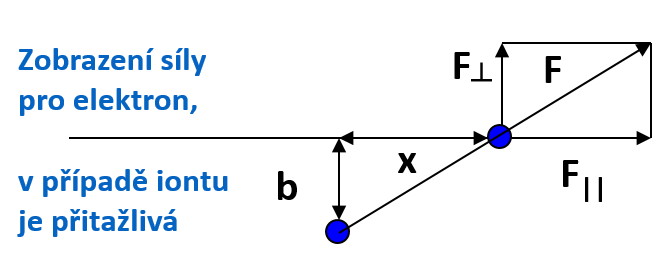
\includegraphics[width=0.6\textwidth]{JS3_bethe.png}
		\captionof{figure}{Zobrazení síly pro elektron, v případě iontu je přitažlivá}		
	\end{center}

	\item Vyjádříme dráhu pomocí rychlosti: $dx = v dt$ 
	Pokud se rychlost $v$ při interakci s jedním elektronem mění málo, je předaná hybnost:
	\begin{equation}
	\begin{gathered}
	\Delta p_b \approx \int_{- \infty}^{+ \infty} \dfrac{F_\perp dx}{v} =  \dfrac{1}{4 \pi \epsilon_0} \dfrac{Z_{ion} e^2 b}{v} \int_{- \infty}^{+ \infty} \dfrac{dx}{(x^2 + b^2)^{3/2}} \\ =  \dfrac{1}{4 \pi \epsilon_0} \dfrac{Z_{ion} e^2 b}{v} \left[ \dfrac{1}{b^2} \dfrac{x}{\sqrt{x^2 + b^2}}\right]_{- \infty}^{+ \infty} = \dfrac{1}{4 \pi \epsilon_0} \dfrac{2 Z_{ion} e^2}{bv}
	\end{gathered}
	\end{equation}
	\item Kinetická energie elektronu po interakci s ionizující částicí:  $E_{KINe} = \dfrac{(\Delta p_{e}^{2})}{2 m_e} = \left( \dfrac{1}{4 \pi \epsilon_0} \right) ^2 \dfrac{2 Z_{ion}^{2}e^4 }{b^2 m_e v^2}$
\end{itemize}
	
Průchod částice materiálem po dráze $\Delta x$:

\begin{itemize}
	\item Mějme tenký cylindr (průřez mezikruží ($b, b + db$)):
	\begin{center}
		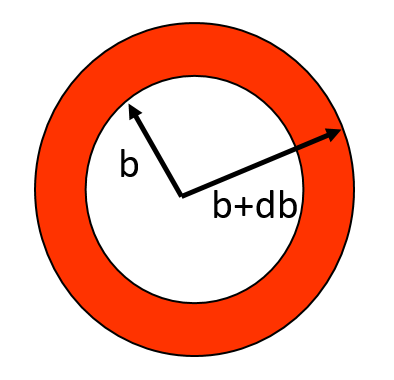
\includegraphics[width=0.3\textwidth]{JS3_mezikruzi.png}
		\captionof{figure}{Infinitezimální obsah mezikruží, kterym prochází částice.}		
	\end{center}
	
	\item Počet elektronů v cylindru: $dN_e = n_e 2 \pi b db \Delta x$,
	kde $n_e$ je hustota elektronů v materiálu
	\item Celková ztráta energie v cylindru: $- \Delta E_{cylindr}  = E_{KINe} \Delta N_e$, kde $\Delta N_e$ je počet elektronů v cylindru
	\item Ztráta energie v celém válci: $- \Delta E = \int E_{KINe} dN_e = n_e \Delta x \int_{0}^{\infty} E_{KINe} 2 \pi b db $
	\item Dosadíme za $E_{KINe}$ : $- \dfrac{dE}{dx} = \left( \dfrac{1}{4 \pi \epsilon_0} \right) ^2\dfrac{4 \pi Z_{ion}^{2} e^4}{m_e v^2} n_e \int_{0}^{\infty} \dfrac{db}{b} $
	\item Je-li náboj atomů materiálu $Z$ platí $n_e = Z n_0$, kde $n_0$ je hustota atomů v materiálu.
	\item Vyjádříme ji pomocí hustoty $\rho$, Avogadrovy konstanty $N_A$ a atomové hmotnosti $A$:
	\begin{equation}
	n_0 = \dfrac{\rho N_A}{A} \Rightarrow n_e = \dfrac{Z}{A} \rho N_A
	\end{equation}
	\item a tedy:
	\begin{equation}
	- \dfrac{dE}{dx} = \left( \dfrac{1}{4 \pi \epsilon_0} \right) ^2 \dfrac{4 \pi Z_{ion}^2 e^4}{m_e v^2} \dfrac{Z}{A} \rho N_A \int_{0}^{\infty} \dfrac{db}{b}
	\end{equation}
	\item V případě limit integrace $0$ a $\infty$  dostáváme divergující integrál.
	\item Limity pro integraci nejsou ve skutečnosti $0$ a $\infty$ , ale $b_{min}$ a $b_{max}$:
	\item Maximální energie je přenesena v čelní srážce, elektron získá energii:
	\begin{equation}
	\Delta E_{MAX} = E_{KINe} (MAX) = \dfrac{1}{2} m_e (2 v)^2
	\end{equation}	
	neboť maximální přenesená hybnost $\Delta p_{MAX} = p_{MAXe} = 2 m_e v$
	\item Použijeme vztah mezi přenesenou energií a parametrem srážky:
	\begin{equation}
	2 m_e v^2 = \left( \dfrac{1}{4 \pi \epsilon_0} \right) ^2 \dfrac{2 Z_{ion}^2 e^4}{b_{MIN}^2 m_e v^2} \Rightarrow b_{MIN} = \left( \dfrac{1}{4 \pi \epsilon_0} \right) \dfrac{2 Z_{ion} e^2}{m_e v^2}
	\end{equation}
	\item Minimální přenesená hybnost závisí na středním ionizačním potenciálu elektronů v atomu $I$ a je rovna $\Delta p _{MIN} = \dfrac{I}{v}$ a $\Delta E_{MIN} = \dfrac{\Delta p_{MIN}^2 }{2 m_e} = \dfrac{I^2}{2 m_e v^2} $ (práce vykonaná při průletu musí být větší než ionizační potenciál) a odpovídající parametr srážky je:
	\begin{equation}
	\dfrac{I^2}{2 m_e v^2} = \left( \dfrac{1}{4 \pi \epsilon_0} \right) ^2 \dfrac{2 Z_{ion}^2 e^4}{b_{MAX}^2 m_e v^2} \Rightarrow b_{MAX} = \left( \dfrac{1}{4 \pi \epsilon_0} \right) \dfrac{2 Z_{ion} e^2}{I} 
	\end{equation}
	\item Určíme příslušný integrál: 
	\begin{equation}
	- \dfrac{dE}{dx} = \left( \dfrac{1}{4 \pi \epsilon_0} \right) ^2 \dfrac{4 \pi Z_{ion}^2 e^4}{m_e v^2} \dfrac{Z}{A} \rho N_A \ln \left( \dfrac{b_{MAX}}{b_{MIN}}\right) 
	\end{equation}
	kde
	\begin{equation}
	\dfrac{b_{MAX}}{b_{MIN}} = \dfrac{\left( \dfrac{1}{4 \pi \epsilon_0} \right) \dfrac{2 Z_{ion} e^2}{I}}{\left( \dfrac{1}{4 \pi \epsilon_0} \right) \dfrac{Z_{ion} e^2}{m_e v^2}} = \dfrac{2 m_e v^2}{I}
	\end{equation}
	\item a tedy:
	\begin{center}
		\hspace*{-1.5cm}
		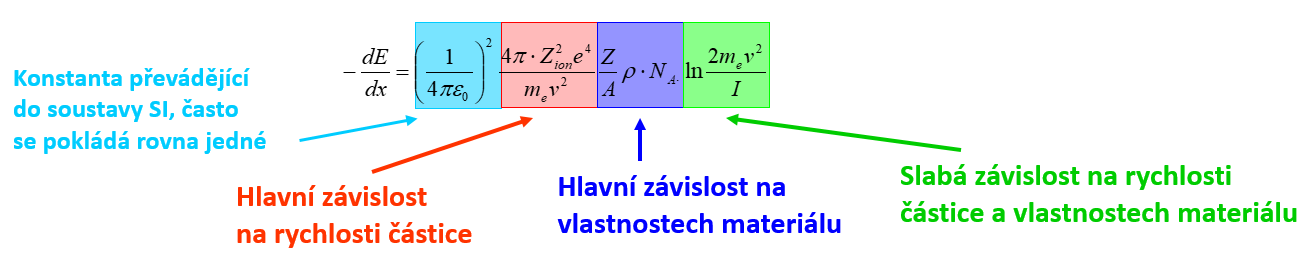
\includegraphics[width=1.05\textwidth]{JS3_bloch.png}
		\captionof{figure}{Bethe-Blochova formule}		
	\end{center}
\end{itemize}

\textbf{RELATIVISTICKÉ OPRAVY:}
\begin{itemize}
	\item Maximální předaná hybnost: $p_{e,max} = 2 mv \Rightarrow p_{e,max} = \dfrac{2mv}{\sqrt{1 - \beta^2 }}$, kde $\beta = \dfrac{v}{c}$
	\item Redukce elektrického pole částice ve směru letu faktorem $(1 - \beta^2)$ a v kolmém směru zvětšení faktorem $1 / \sqrt{1 - \beta^2}$
	\item Nakonec dostaneme:
	\begin{equation}
	- \dfrac{dE}{dx} =  \left( \dfrac{1}{4 \pi \epsilon_0} \right) ^2 \dfrac{4\pi Z_{ion}^2 e^4}{m_e c^2 \beta^2} \dfrac{Z}{A} \rho N_A \left[\ln \left( \dfrac{2 m_e c^2 \beta^2 }{I}\right) + \ln \left(\dfrac{1}{1 - \beta^2} \right)  - \beta^2 \right] 
	\end{equation}
	\begin{equation}
	- \dfrac{dE}{dx} = \left( \dfrac{1}{4 \pi \epsilon_0} \right) ^2 \dfrac{4\pi Z_{ion}^2 e^4}{m_e c^2 \beta^2} \dfrac{Z}{A} \rho N_A \left[\ln \left( \dfrac{2 m_e c^2 \beta^2}{I(1- \beta^2)}\right) - \beta^2 \right] 
	\end{equation}
	\item Pro $v \ll c$ dostaneme dříve uvedenou rovnost.
\end{itemize}

Pro elektrony je tato rovnost ještě složitější:
\begin{itemize}
	\item V případě elektronu $\rightarrow$ identické částice $\rightarrow$ maximální předaná energie $\Delta E_{MAX} E/2$
	\begin{equation}
	\begin{gathered}
	- \dfrac{dE}{dx} = \left( \dfrac{1}{4 \pi \epsilon_0} \right) ^2 \dfrac{4\pi Z_{ion}^2 e^4}{m_e c^2 \beta^2} \dfrac{Z}{A} \rho N_A \dfrac{1}{2} \left[ \ln \dfrac{m_e c^2 \beta^2 E}{2 I^2 (1 - \beta^2)} - (\ln 2) (2\sqrt{1 - \beta^2} - 1 + \beta^2) \right. \\ \left. + (1 - \beta^2) + \dfrac{1}{8} (1 - \sqrt{1 - \beta^2}) ^2 \right] 
	\end{gathered}
	\end{equation}
\end{itemize}

\begin{center}
	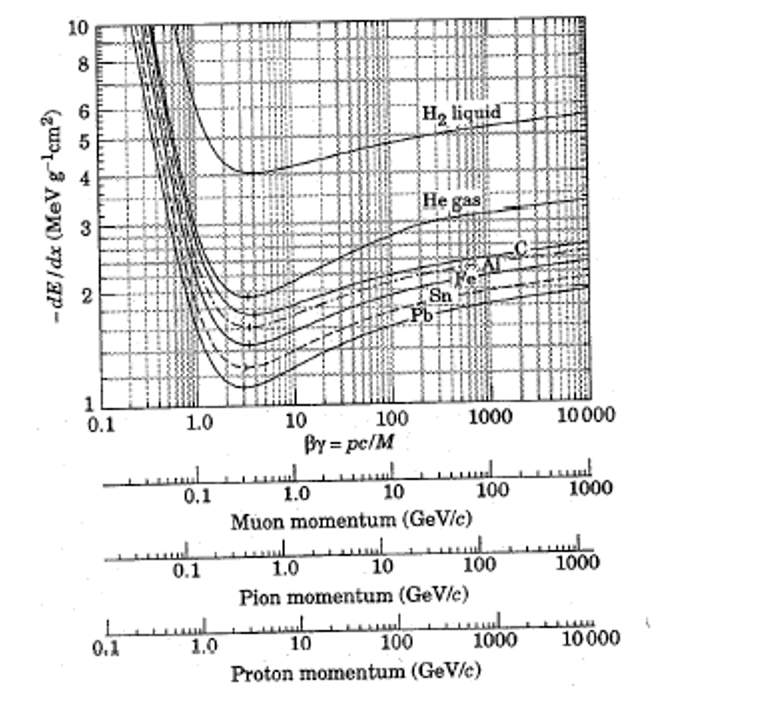
\includegraphics[width=0.7\textwidth]{JS3_ztraty.png}
	\captionof{figure}{Ukázka ionizačních ztrát pro  některé částice }		
\end{center}

Porovnáme-li ztráty ionizací pro elektron a pro těžké nabité částice téže kinetické energie, zjistíme, že při nízkých energiích (stovky $\mathrm{MeV}$) jsou ztráty těžkých nabitých částic asi 1000-krát větší. Při relativistických energiích (řádově $\mathrm{GeV}$) jsou ale ztráty elektronů se ztrátami těžkých částic srovnatelné. Proto v dráhových detektorech jsou stopy těžkých nabitých částic nízkých energií tlustší než stopy elektronů, zatímco při relativistických energiích vykazují stopy všech nabitých částic stejnou tloušťku.

\subsection{Pružný rozptyl}

\begin{itemize}
	\item Jednotlivý rozptyl $d \ll \dfrac{1}{n_0 \sigma}$
	\item Násobný rozptyl $d \sim \dfrac{1}{n_0 \sigma}$
	\item Mnohonásobný rozptyl $d \gg \dfrac{1}{n_0 \sigma}$	
\end{itemize}

\begin{itemize}
	\item Těžké částice - významný jen rozptyl na atomových jádrech
	\item Lehké částice - významný i rozptyl na elektronech
\end{itemize}

Jednotlivý rozptyl v poli jádra - popsán pomocí Rutherfordova rozptylu:
\begin{equation}
\cot \left( \dfrac{\vartheta}{2}\right) = \dfrac{4 \pi \epsilon_0 m v^2 b}{Z_{ion} Z e^2}
\end{equation}

\begin{itemize}
	\item Těžké částice - rozptyl na malé úhly $\rightarrow$ dráha lehce zvlněná
	\item Lehké částice - rozptyl na velké úhly $\rightarrow$ nedefinovaný dolet (pro \quotedblbase nižší energie\textquotedblright)
\end{itemize}

Střední kvadratická odchylka od původního směru $\overline{\varTheta ^2}$ závisí na střední kvadratické hodnotě úhlu rozptylu $\overline{\vartheta ^2}$: 

(zjednodušené klasické odvození pro \quotedblbase těžké částice\textquotedblright ~- malé úhly rozptylu)

\begin{itemize}
	\item $\vartheta \rightarrow 0$: 
	\begin{equation}
	\dfrac{\vartheta}{2} \approx \tan \left( \dfrac{\vartheta}{2} \right) = \dfrac{Z_{ion} Z e^2}{4 \pi \epsilon_0 m v^2 b} 
	\end{equation}
	a tedy:
	\begin{equation}
	\vartheta ^2 \approx \dfrac{(Z_{ion} Z e^2)^2}{4 (\pi \epsilon_0 m v^2 )^2 b^2}
	\end{equation}
	\item Určíme $\overline{\vartheta ^2}$:
	\begin{equation}
	\begin{gathered}
	\overline{\vartheta ^2} = \dfrac{\int_{b_{min}}^{b_{max}} \vartheta ^2 (b) 2 \pi b db}{\int_{b_{min}}^{b_{max}} 2 \pi b db} = \dfrac{\dfrac{2 \pi (Z_{ion} Z e^2)^2}{4 (\pi \epsilon_0 m v^2)^2} \int_{b_{min}}^{b_{max}} \dfrac{1}{b}db}{2 \pi \int_{b_{min}}^{b_{max}}b db} = \dfrac{\dfrac{ \pi (Z_{ion} Z e^2)^2}{2 (\pi \epsilon_0 m v^2)^2} [\ln b]_{b_{min}} ^{b_{max}}}{\pi [b^2]_{b_{min}}^{b_{max}}}\\  = \dfrac{\left( \dfrac{Z_{ion} Z e^2}{\pi \epsilon_0 m v^2}\right)^2 \ln \dfrac{b_{max}}{b_{min}} }{2 (b_{max}^2 - b_{min}^2)}
	\end{gathered}
	\end{equation}
	\item $\overline{\varTheta ^2}$ je pak určeno: 
	\begin{equation}
	\overline{\varTheta ^2} = N_{roz} \overline{\vartheta ^2} 
	\end{equation}
	kde $N_{roz}$ je počet rozptylů:
	\begin{equation}
	N_{roz} = N_{atom} x \sigma = \rho \dfrac{N_A}{A} x \int_{b_{min}}^{b_{max}} 2 \pi b db = \pi \rho \dfrac{N_A}{A} x (b_{max}^2-b_{min}^2) 
	\end{equation}
	\item Výsledná hodnota je:
	\begin{equation}
	\overline{\varTheta ^2} = \dfrac{1}{2} 	\rho \dfrac{N_A}{A} x \pi \left(\dfrac{Z_{ion} Z e^2}{\pi \epsilon_0 m v^2} \right)^2 \ln \dfrac{b_{max}}{b_{min}} = \dfrac{1}{2 \pi \epsilon_{0}^2} \rho \dfrac{N_A}{A} \dfrac{x Z_{ion} ^2 Z^2 e^4}{p^2 v^2} \ln \dfrac{b_{max}}{b_{min}}
	\end{equation}
\end{itemize}

Důležité vlastnosti rozptylu:
\begin{itemize}
	\item Silná závislost na hybnosti
	\item Silná závislost na rychlosti: $1/v^4$
	\item Silná závislost na hmotnosti: $1/m^2$
	\item Silná závislost na náboji částice: $Z_{ion}^2$
	\item Silná závislost na $Z$ prostředí: $Z^2$
\end{itemize}

\subsection{Brzdné záření}

Ztráty energie buzením brzdného záření nazýváme radiačními ztrátami. K buzení brzdného záření letící nabitou částicí dochází v poli atomového jádra, resp. v poli obalového elektronu, v důsledku vzájemného coulombického působení. Nabitá částice ztratí část své kinetické energie, která se vyzáří ve formě fotonů. Částice přitom změní směr své dráhy, jak lze vidět na Obr. \ref{js3:obr:JS3_brzda}. 

\begin{figure}
	\centering
	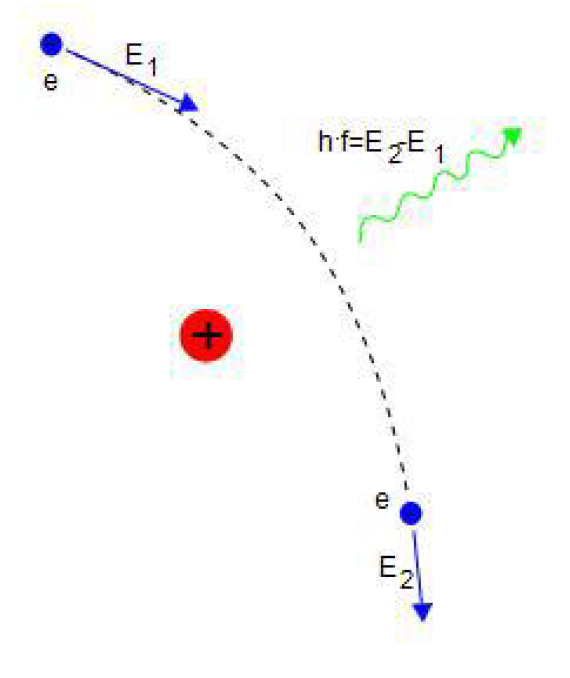
\includegraphics[width=0.3\textwidth]{JS3_brzda.png}
	\caption{Brzdné záření produkované nalétávajícím vysokoenergetickým elektronem v poli atomového jádra}	
	\label{js3:obr:JS3_brzda}	
\end{figure}

Nabitá částice pohybující se zrychleně vyzařuje elektromagnetické záření.

\begin{itemize}
	\item Energie vyzářená za časovou jednotku: $ - \dfrac{dE}{dt} \sim a^2$
	\item Zrychlení je dáno Coulombovou interakcí:
	\begin{equation}
	\left| a \right| = \dfrac{\left| F_c \right| }{m} = \dfrac{1}{4 \pi \epsilon_0} \dfrac{Z_{ion} Z e^2}{r^2} \dfrac{1}{m}
	\end{equation}
	\item Závislost na náboji prostředí: $- \dfrac{dE}{dt} \sim Z^2 $, závislost na náboji iontu: $- \dfrac{dE}{dt} \sim Z_{ion}^2$ 
	
	a hmotnosti: $- \dfrac{dE}{dt} \sim \dfrac{1}{m^2}$
	\item Rozdíl v náboji iontu malý, v hmotnosti mnohem větší:
	\item Pro proton a elektron:
	\begin{equation}
	\dfrac{\left( - \dfrac{dE}{dt}\right)_{rad} (proton)}{\left( - \dfrac{dE}{dt}\right)_{rad} (elektron)} = \dfrac{\dfrac{1}{m_{p}^2}}{\dfrac{1}{m_{e}^2}} = \dfrac{m_{e}^2}{m_{p}^2} = \left(\dfrac{0,511 ~\mathrm{MeV}}{938 ~\mathrm{MeV}} \right) ^2 = 0,3\cdotp 10^{-6}
	\end{equation}
	\item Pro mion a elektron je stejný poměr $2,6 \cdotp 10^{-5}$
\end{itemize}

Radiační ztráty se projevují v \quotedblbase normální\textquotedblright ~situaci jen u elektronu a pozitronu. Při ultrarelativistických energiích i pro další částice. Platí tedy, že radiační ztráty jsou nejvyšší u nejlehčích částic (protonů a pozitronů). Ztráty energie buzením brzdného záření jsou úměrné kvadrátu atomového čísla látky, nejvýraznější jsou tedy v látkách s těžkými atomy.

Radiační ztráty se vedle ionizačních ztrát začínají uplatňovat v lehkých látkách při kinetických energiích elektronů $T \geq 100 ~\mathrm{MeV}$, v těžkých látkách při $T \geq 10 ~\mathrm{MeV}$.

\begin{itemize}
	\item Na základě kvantové fyziky dostaneme pro ztráty energie pro elektron (pozitron) $Z_{ion} = 1$:
	\item Popis ekvivalentní popisu tvorby párů:
	\item (jde o podobný výpočet i výsledek jako pro produkci párů - viz interakce záření $\gamma$)
	\begin{equation}
	\left( - \dfrac{dE}{dx}\right) _{rad} = 4 \rho \dfrac{N_A}{A} r_{0}^2 \alpha E Z^2 F(E,Z) 
	\end{equation}
	kde pro připomenutí:
	\begin{equation}
	r_0 = \dfrac{e^2}{4 \pi \epsilon_0 m_e c^2} = 2,82 \cdotp 10^{-15} ~\mathrm{m}, ~~ ~~~~ \alpha = \dfrac{e^2}{4 \pi \epsilon_0 \eta c} = \dfrac{1}{137} 
	\end{equation}
	\item průběh funkce $F(E,Z)$ závisí na energii ($E_0$ - počáteční energie elektronu) - zda je nutno započíst stínění elektronů:
	\item $E \approx h \nu_0$ - vlastní frekvence atomu $\rightarrow$ interakce s atomem - není vliv stínění
	\item $E \gg h \nu_0$ - interakce s jádrem $\rightarrow$ stínění je zapotřebí započíst podle toho, kde elektron s jádrem interaguje:
	\begin{itemize}
		\item Malá energie $\rightarrow$ nutno velké pole blízko jádra
		\item Velká energie $\rightarrow$ stačí slabé pole dál od jádra - tam je maximum produkce
		\begin{itemize}
			\item bez stínění: $m_e c^2 \ll E_0 \ll \dfrac{m_e c^2 Z^{1/3}}{\alpha}$: ~~~$F(E,Z) = \ln 2 \xi - f(Z) - \dfrac{1}{3}$,~~~ kde $\xi = \dfrac{E_0}{m_e c^2}$
			\item úplné stínění: $E_0 \gg \dfrac{m_e c^2 Z^{1/3}}{\alpha}$: ~~~$F(E,Z) = \ln(183 Z^{-1/3})- f(Z) + \dfrac{1}{18}$
		\end{itemize}	
    \end{itemize}
  a $F(E,Z)$ v případě bez stínění slabě závisí na $E$ a v případě úplného stínění na $E$ nezávisí . 	
\end{itemize}
 
\textbf{Vztah pro ztráty energie brzdným zářením} (Bethe-Heitlerův vztah): 
\begin{equation}
\left(- \dfrac{dE}{dx} \right) _{rad} = \dfrac{1}{X_0} E
\end{equation}

\begin{itemize}
	\item Pro radiační délku $X_0$ pak platí: $\dfrac{1}{X_0} = 4 \rho \dfrac{N_A}{A} r_{0}^2 \alpha Z^2 F(E,Z)$
	\item Energetické ztráty elektronu (jsou-li pouze radiační ztráty): $E(x) = E_0 \exp \left(-\dfrac{x}{X_0} \right)$
	kde $E_0$ je počáteční kinetická energie elektronů a $x$ je tloušťka absorbátoru.
\end{itemize}

Jak je vidět, kinetická energie elektronů klesá při průchodu prostředím exponenciálně. Navíc nám tento vztah poskytuje i fyzikální význam radiační délky $X_0$ - je to úsek dráhy, na kterém energie elektronů poklesne na $1/e$. Termín brzdného záření byl zaveden Nikolou Teslou.

\textbf{Energetické spektrum fotonů brzdného záření}:

Energii fotonů lze vypočítat pomocí vztahu $E_{\gamma} = h \nu_0$. Frekvenci získáme jako $\nu_0 = \dfrac{1}{h} (E - m_e c^2)$. 

\begin{center}
	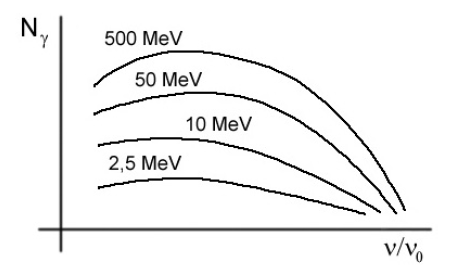
\includegraphics[width=0.7\textwidth]{JS3_fotony.png}
	\captionof{figure}{Energetické spektrum fotonů brzdného záření}		
\end{center}
 	
\textbf{Porovnání ionizačních a radiačních ztrát}:
\begin{itemize}
	\item Kritická energie $E_c$: $ E = E_c$ $\Rightarrow \left( \dfrac{dE}{dx}\right) _{rad} = \left(\dfrac{dE}{dx} \right)_{ion}$
	\item Pro elektron a pozitron je $E_c > m_e c^2$ $\rightarrow v \approx c$
	\begin{equation}
	\left(- \dfrac{dE}{dx}\right) _{rad} = \left(- \dfrac{dE}{dx} \right)_{ion} \Leftrightarrow 4 \rho \dfrac{N_A}{A} r_{0}^2 \alpha E Z^2 F_{rad} (E,Z) = \left( \dfrac{1}{4 \pi \epsilon_0} \right)^2 \dfrac{4 \pi e^4 }{m_e c^2} \dfrac{Z}{A} \rho N_A F_{ion} (E)
	\end{equation}
	\begin{equation}
	\dfrac{	\left(- \dfrac{dE}{dx}\right) _{rad}}{\left(- \dfrac{dE}{dx} \right)_{ion}} = \dfrac{\alpha}{\pi} \dfrac{E}{m_e c^2} Z \dfrac{F_{rad} (E,Z)}{F_{ion}(E)} = \dfrac{\alpha}{\pi} \xi Z \dfrac{F_{rad} (E,Z)}{F_{ion}(E)} \approx \dfrac{ZE}{1600 m_e c^2}
	\end{equation}
	\item Rovnost ionizačních a radiačních ztrát nastává při 
	\begin{equation}
	E_c \approx \dfrac{1600 m_e c^2}{Z}
	\end{equation}
	\item pro $v \rightarrow c$ platí $F_{ion}(E) = f(\ln E)$:
	\begin{equation}
	\xi _ c = \dfrac{E_c}{m_e c^2} = \dfrac{\pi}{\alpha} \dfrac{1}{Z} \dfrac{F_{ion}(E)}{F_{rad}(E,Z)}
	\end{equation}
\end{itemize}

\begin{center}
	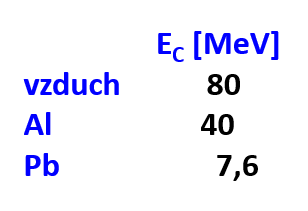
\includegraphics[width=0.2\textwidth]{JS3_krit.png}
	\captionof{figure}{Kritická energie}		
\end{center}
 
\subsection{Celkové ztráty energie}

Celkové energetické ztráty elektronu jsou rovny součtu ionizačních a radiačních ztrát:
\begin{equation}
\left( - \dfrac{dE}{dx}\right)_{celkové} = \left( - \dfrac{dE}{dx}\right)_{ion} + \left( - \dfrac{dE}{dx}\right)_{rad} 
\end{equation}

\begin{center}
	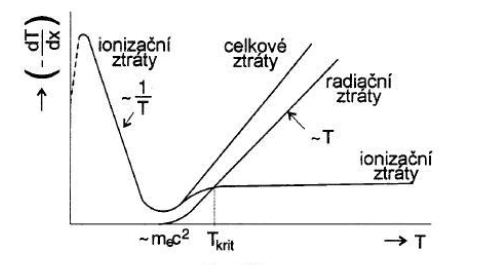
\includegraphics[width=0.7\textwidth]{JS3_celk.png}
	\captionof{figure}{Ztráty energie elektronu při průchodu látkou}		
\end{center}

Vidíme, že do hodnoty $E \approx m_e c^2$ se celkové ztráty rovnají ionizačním ztrátám. Od této energie jsou celkové ztráty dány jako součet ionizačních a radiačních ztrát. pro energie $E > E_c$ převládají radiační ztráty.

\subsection{Dosah elektronů v látce, pohlcení}

Elektron se může při jedné srážce výrazně odchýlit od své původní dráhy. Proto dráha elektronu, na rozdíl od těžké nabité částice, je v látce křivočará a její celková délka je podstatně větší než je dosah elektronů. Na Obr. \ref{js3:obr:elektrony} je absorbční křivka znázorňující závislost počtu monoenergetických elektronů na tloušťce absorbátoru. Neexistuje přesný dosah.

 \begin{center}
 	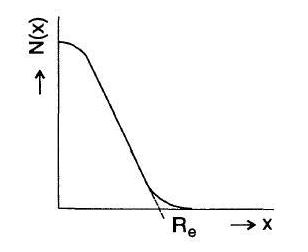
\includegraphics[width=0.5\textwidth]{JS3_elektrony.png}
 	\captionof{figure}{Dosah elektronů v látce \label{js3:obr:elektrony}}		
 \end{center}

Ze závislosti vidíme, že počet elektronů klesá téměř lineárně s tloušťkou absorbátoru. Pokud prodloužíme lineární část k ose $x$, dostaneme tzv. extrapolovaný dosah $R_e$. Tato veličina udává tloušťku absorbátoru, jež zadrží všechny elektrony (proto je $R_e$ někdy nazýváno maximálním dosahem).

Teoreticky počítat hodnoty $R_e$ je velmi obtížné (vzhledem k tomu, že trajektorie není přímočará, nelze integrovat jako v případě těžkých nabitých částic). Proto se zde používají opět empirické vztahy:
\begin{itemize}
	\item pro hliník (hliník je uváděn proto, že má vhodné vlastnosti, např. u elektronů nevyvolává brzdné záření):
	\begin{equation}
	R_e [\mathrm{g\cdotp cm^{-2}}] = 0,407 T^{1,38} , ~~~~~ 0,15 ~\mathrm{MeV} < T < 0,8 ~\mathrm{MeV},
	\end{equation}
	\begin{equation}
	R_e = 0,542 T - 0,133, ~~~~~0,8 ~\mathrm{MeV} < T < 3 ~\mathrm{MeV}
	\end{equation}
	\item pro jiné prvky: 
	\begin{equation}
	R_X = R_{Al} \dfrac{(Z/A)_{Al}}{(Z/A)_X}
	\end{equation}
\end{itemize}	
	
Pro spektrum zářiče $\beta$ dostaneme exponenciální závislost.

\begin{center}
	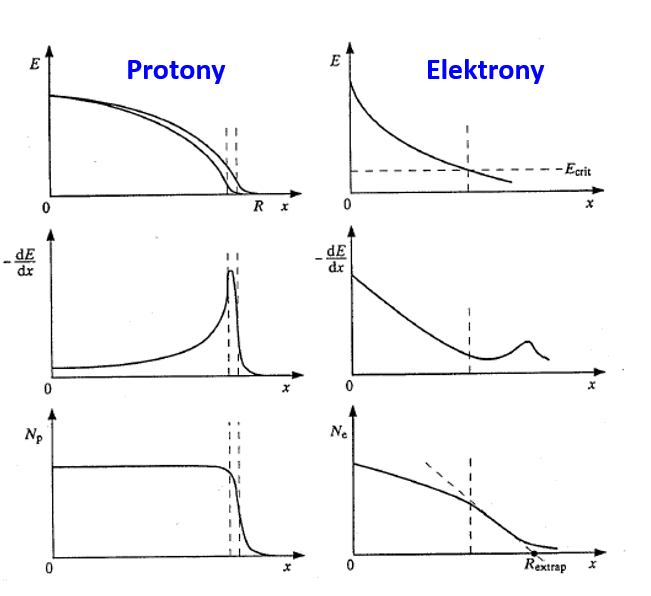
\includegraphics[width=0.7\textwidth]{JS3_dosah.png}
	\captionof{figure}{Schématické porovnání různých veličin pro protony a elektrony}		
\end{center}

\subsection{Elektromagnetická kaskáda (sprška)}

Elektromagnetická sprška vzniká u vysoce energetických elektronů nebo $\gamma$-kvant. Při dostatečně vysoké energii totiž může foton způsobit generaci elektron-pozitronového páru. Stejně tak elektron s dost vysokou energií způsobuje brzdné záření o vysoké energii.

Proces je rozkreslen na Obr.\ref{js3:obr:sprska} - elektron se zbrzdí (a odkloní) vysláním $\gamma$-kvanta, to dále generuje pár $e^+ e^-$, který se potenciálně může dále brzdit vysíláním brzdného záření.

\begin{center}
	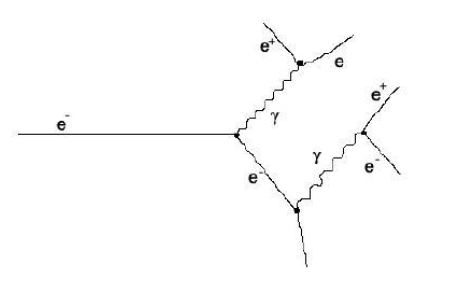
\includegraphics[width=0.6\textwidth]{JS3_sprska.png}
	\captionof{figure}{Elektromagnetická sprška \label{js3:obr:sprska}}		
\end{center}

\subsection{Ultrarelativistické energie}

\begin{center}
	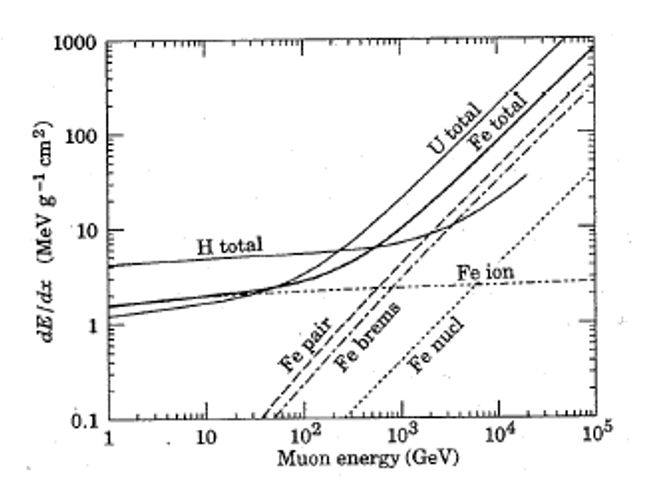
\includegraphics[width=0.6\textwidth]{JS3_radiace.png}
	\captionof{figure}{Při ultrarelativistické energii převládnou i u mionů radiační ztráty brzdným zářením a produkcí párů}		
\end{center}

\subsection{Úhlové a energetické rozdělení fotonů brzdného záření}

\begin{itemize}
	\item Úhlové rozdělení - úhlové rozdělení vysílaných fotonů brzdného záření závisí na energii nabitých částic, nezávisí na energii vysílaných fotonů. Střední úhel $\varTheta$ emise kvant brzdného záření, buzeného elektrony s energií $E_{TOT}$, je přibližně dán vztahem
	\begin{equation}
	\sim \varTheta_S = \dfrac{m_e c^2}{E_{TOT}} = \gamma ~~~~~~~~~~~~~~ E \longrightarrow \infty \Rightarrow \varTheta_S \longrightarrow 0
	\end{equation}
	
	Při nízkých energiích je brzdné záření vyzařováno prakticky izotropně do všech směrů od míste interakce. Se vzrůstající energií $E$ elektronu budícího brzdné záření je střední úhel $\varTheta_S$ emitovaných fotonů stále menší. Při vysokých energiích dopadajících nabitých částic je brzdné záření přednostně vysíláno v úzkém kuželu \quotedblbase vpřed\textquotedblright ~(v dopředném směru) ve směru dopadu nabitých částic.
	
	\item Energetické rozdělení - maximální možná vyzářená energie - kinetická energie elektronu
\end{itemize}	

\subsection{Výkon brzdného záření}

Nyní uvedeme vztahy pro výkon brzdného záření na tenkém a ne přliš tlustém terčíku:
\begin{itemize}
	\item Tenký terčík: $P_{rad} = 1,9 \cdotp 10^3 (T + m_e c^2) \frac{Z \rho d I}{A}$, přičemž jsme zanedbali ionizační ztráty a mnohonásobný rozptyl
	\item Ne příliš tlustý terčík: $P_{rad} = 3\cdotp10^{-3} T^{1,75} Z I$, kde předpokládáme, že se elektron v terči zabrzdí, ale ne natolik, aby ztratil veškerou svou energii
	
Při tom $d$ je tloušťka terčíku, $I$ je proud elektronů a $\rho$ je hustota látky, ze které je terčík vyroben.	
\end{itemize}

\subsection{Absorbce záření $\beta$}

Zářiče $\beta$ emitují záření se spojitým energetickým spektrem. Nízkoenergetické $\beta$-záření jsou absorbovány již v malých tloušťkách absorbátoru, většina ze spektra $\beta$-záření má však přibližně exponenciální dosah (toto chování je však pouze empirická aproximace, která nemá fundamentální základy jako je tomu například u exponenciálního útlumu $\gamma$- záření).

\begin{center}
	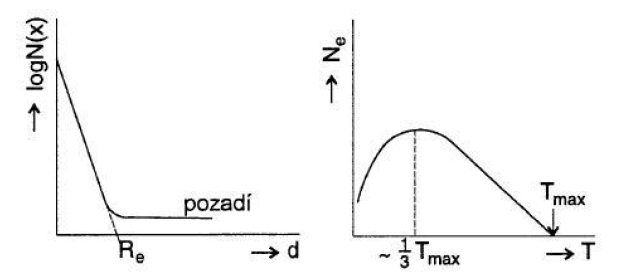
\includegraphics[width=0.6\textwidth]{JS3_beta.png}
	\captionof{figure}{Vlevo: dosah $\beta$-záření, vpravo: spektrum $\beta$-záření}		
\end{center}

Produkci $\beta$-záření lze popsat procesem
\begin{equation}
^{A}_{Z}X \rightarrow ^{A}_{Z+1}X + e^- + \overline{\nu},
\end{equation}
kde $\overline{\nu}$ je antineutrino. Součet energií $e^- + \overline{\nu}$ je pokaždé stejný, ovšem rozdělení energie mezi těmito dvěma částicemi může být různé.

Dosah $\beta$-záření lze popsat vzorcem
\begin{equation}
N(d) = N_0 \exp (- \mu d),
\end{equation}
kde $N_0$ je počet elektronů před vstupem do absorbátoru, $N(d)$ je počet elektronů, které prošly tloušťkou absorbátoru $d$ a $\mu$ je lineární součinitel zeslabení. Zavádí se též hmotnostní součinitel zeslabení $\mu_m = \mu /\rho $, kde $\rho$ je hustota absorbátoru. Veličina $\mu_m$ závisí na $E_{max}$ a mění se jen málo s atomovým číslem $Z$ jader absorbátoru. To dovoluje aproximovat empirickou formulí
\begin{equation}
\mu _m [\mathrm{cm^2 \cdotp g}] \approx \dfrac{22}{T_{max}^{4/3} [\mathrm{MeV}]}
\end{equation}

\subsection{Synchrotronové záření}

Zvláštním druhem brzdného záření, je tzv. synchrotronové záření. Vzniká při pohybu relativistických nabitých částic v magnetickém poli, kde na tyto částice působí Lorentzova síla zakřivující jejich dráhy. V důsledku nerovnoměrného pohybu elektricky nabitých částic při kruhovém oběhu pod vlivem magnetického pole pak vzniká brzdné záření. Vzniká na kruhových urychlovačích, tzv. synchrotronech. 

Intenzita synchrotronového záření je úměrná elektrickému náboji a druhé mocnině zrychlení pohybu částice, naproti tomu je nepřímo úměrná kvadrátu  hmotnosti částice (proto se uplatňuje zejména u lehkých částic o vysokých energiích).

Synchrotronové záření není spojeno s látkou - čím menší zrychlení, tím nižší je jeho energie.

\begin{itemize}
	\item Působící síla je Lorentzova síla: $\vec F_L = q (\vec v \times \vec B)$
	\item Ztráty energie: $- \dfrac{dE}{dt} = \dfrac{2}{3} \dfrac{1}{4 \pi \epsilon_0} \dfrac{(Ze)^2}{c^3} \left| \vec a \right| ^2$
	\item Klasické dostředivé zrychlení: $a = v^2 /R$
	\begin{itemize}
	\item Ztráty energie: $- \dfrac{dE}{dt} = \dfrac{2}{3} \dfrac{1}{4 \pi \epsilon_0} \dfrac{(Ze)^2}{c^3} \dfrac{v^4}{R^2}$
	\end{itemize}
\item Relativistické dostředivé zrychlení: $a = \dfrac{1}{m} \dfrac{dp}{d\left(\dfrac{t}{\gamma}\right) } = \dfrac{\gamma}{m} \left( \dfrac{d(\gamma m) v}{dt} \right) = \gamma^2 \dfrac{dv}{dt} =  \gamma^2 \dfrac{v^2}{R}$
\begin{itemize}
	\item Ztráty energie: $- \dfrac{dE}{dt} = \dfrac{2}{3} \dfrac{1}{4 \pi \epsilon_0} \dfrac{(Ze)^2}{c^3} \left| \gamma^2 \dfrac{v^2}{R} \right| = \dfrac{2}{3} \dfrac{1}{4 \pi \epsilon_0} \dfrac{(Ze)^2}{c^3} \gamma ^2 \dfrac{v^4}{R^2} =  \dfrac{2}{3} \dfrac{1}{4 \pi \epsilon_0} \dfrac{(Ze)^2}{R^2} c \gamma^4 \beta^4$,
	
	kde $\gamma^2 = \dfrac{1}{1 - \beta^2}.$
\end{itemize}
\end{itemize}

\subsection{Čerenkovovo záření}

Čerenkovovo záření vzniká tehdy, pokud se nabitá částice pohybuje v optickém prostředí rychlostí větší, než je fázová rychlost světla v daném prostředí ($v > c' = c/n$, kde $n$ je index lomu prostředí).

Při průchodu elektricky nabité částice látkovým prostředím dochází k místní polarizaci atomů a molekul podél dráhy. Po průchodu částice se atomy samy opět depolarizují, přičemž získanou energii vyzařují ve formě elektromagnetického záření. To podléhá interferenci, jejíž výsledek závisí na rychlosti částice. Je-li rychlost pohybu částice v prostředí větší, než je  fázová rychlost světla, mohou se elektromagnetické vlny, které vznikají v různých místech dráhy, dostat do fáze a ve vhodném úhlu $\varTheta$ se tyto fáze mohou sečíst za vzniku pozorovatelného záření.

Každé místo dráhy částice se vlivem depolarizace prostředí stává zdrojem slabého elektromagnetického záření, jež se šíří rychlostí $c/n$. Za čas $t$ se záření rozšíří do kulové vlnoplochy o poloměru $ct/n$. Nabitá částice za tentýž čas urazí vzdálenost $\beta ct$, kde $\beta = v/c$. Během tohoto časového intervalu se od dalších bodů dráhy postupně rozbíhají kulové vlnoplochy. Společná obálka těchto vlnoploch tvoří plášť kužele. 

\begin{figure}[h!]
	\begin{subfigure}[c]{0.5\linewidth}
		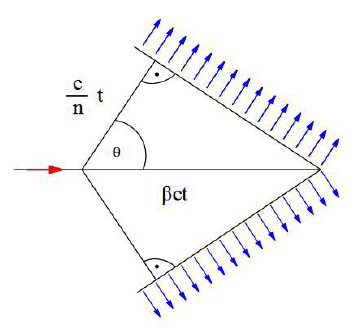
\includegraphics[width=\linewidth]{JS3_cerenko2.png}
		\caption{Řez kuželem, který vytváří společná obálka kulových vlnoploch}
	\end{subfigure}
	\begin{subfigure}[c]{0.5\linewidth}
		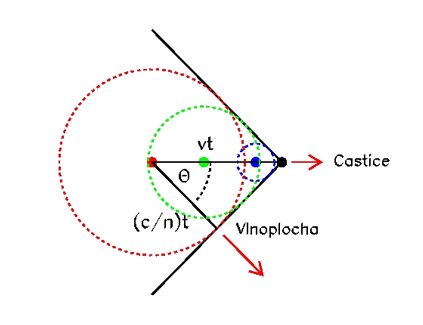
\includegraphics[width=\linewidth]{JS3_cerenko.png}
		\caption{Nákres Čerenkovova záření}
	\end{subfigure}
	\caption{Čerenkovovo záření}
\end{figure}

V řezu tohoto kužele lze nalézt pravoúhlý trojúhelník, z něhož vyplývá, že zesilující interference bude nastávat pod úhlem $\varTheta$, pro nějž lze psát
\begin{equation}
\cos \varTheta = \dfrac{\frac{c}{n} t }{v t} = \dfrac{1}{n \beta}
\end{equation}

Pod tímto úhlem se také vzniklé záření kuželovitě rozbíhá od dráhy letící nabité částice.

Z tohoto vztahu plyne:
\begin{itemize}
	\item Existuje prahová rychlost $\beta_{min} = 1/n$. Pro $\beta_{min}$ jde vyzařování ve směru pohybu částice. Pro nižší rychlost Čerenkovovo záření nevznikne.
	\item Pro ultrarelativistické částice $\cos \varTheta _{max} = 1/n$
	\item Pro vodu: $n = 1,33 \rightarrow \beta_{min} = 0,75$, pro elektron $E_{KIN} = 0,26 ~\mathrm{MeV}$, $\cos \varTheta _{max} = 0,75 \rightarrow \varTheta_{max} = 41,5 ^\circ$ 
\end{itemize}

Jelikož kosinus úhlu může být maximálně roven jedné, dostáváme minimální rychlost letící nabité částice pro produkci Čerenkovova záření $v_{min} = c/n$. Pro úhel $\varTheta = 0^{\circ}$ a vyzařování jde ve směru pohybu částice.

Minimální rychlosti potřebné k vyzařování Čerenkovova záření odpovídají prahové kinetické energii částice (kde $\beta_{min} = v_{min}/c$)
\begin{equation}
E_{min} = m_0 c^2 \left( \dfrac{1}{\sqrt{1 - \beta_{min}^2}} - 1\right) 
\end{equation}

Počet fotonů vzniklých na dráze délky $l$ s vlnovou délkou $\lambda \in (\lambda _1, \lambda_2) $ je určen vztahem
\begin{equation}
N(\lambda_1, \lambda_2) = \dfrac{2 \pi Z^2}{137} l \left( \dfrac{1}{\lambda_1} - \dfrac{1}{\lambda_2}\right) \sin^2 (\varTheta)
\end{equation}

Nakonec uvedeme základní rozdíly mezi brzdným zářením a Čerenkovovým zářením:
\begin{itemize}
	\item Čerenkovovým zářením je viditelné světlo nebo UV záření, kdežto brzdným zářením vzniká foton s energií úměrnou nabité částici (tj. nejedná se o viditelné záření)
	\item Čerenkovovo záření se šíří pouze na vlnoplochách, kdežto brzdné záření vyplňuje celý kužel.
\end{itemize}

\subsection{Přechodové záření}

Při průchodu nabité částice rozhraním mezi materiály s různým indexem lomu $\rightarrow$ emise elektromagnetického záření (objev Ginsburg, Frank 1946).

Vytvoření dipólu v hraniční zóně $\rightarrow$ dipól, elektromagnetické pole se mění v čase $\rightarrow$ emise elmag. záření:
\begin{itemize}
	\item Energie vyzářená na jeden přechod látka/vakuum:
	\begin{equation}
	E = \dfrac{1}{3} \alpha \eta \omega_p \gamma \sim \gamma
	\end{equation}
	\item Vysokoenergetický elektron vyzařuje přechodové záření 
	\item plazmová frekvence: $\hbar \omega_p \approx 14 ~\mathrm{MeV}$ (pro $Li$), $0,7 ~\mathrm{eV}$ (vzduch), $20 ~\mathrm{eV}$ (polyethylen)
	\item Počet fotonů vyzářených na hranici (je velmi malý, potřeba hodně přechodů):
	\begin{equation}
	N_f = \dfrac{E}{<\eta \omega >} \sim \gamma 
	\end{equation}
	\item Energie vyzářených fotonů: $10 - 30 ~\mathrm{keV}$ 
	\item $N_f \sim \dfrac{1}{3} \dfrac{1}{137} \dfrac{20 ~\mathrm{eV}}{20000 ~\mathrm{eV}} \gamma \sim 0,000002 \gamma$
	\item Vyzařování ostře směřováno ve směru letu částice: $\varTheta \sim \dfrac{1}{\gamma}$
\end{itemize}

\begin{center}
	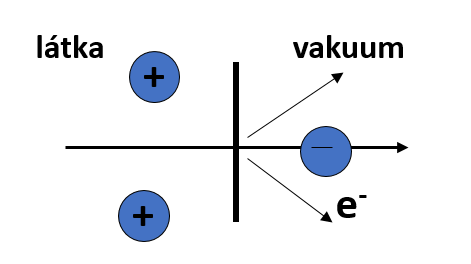
\includegraphics[width=0.6\textwidth]{JS3_prechod.png}
	\captionof{figure}{Přechodové záření}		
\end{center}

Radiátory přechodového záření: materiál s malým $Z$, reabsorbce roste s $ \sim Z^5$. Dobrá kombinace radiátorů a rentgenových detektorů.

\section{Detektory a spektrometry lehkých nabitých částic}
	
Nutnost detekce v širokém rozsahu energií:
\begin{itemize}
	\item Atomová fyzika - $\mathrm{meV} - ~\mathrm{eV}$
	\item Augerovy elektrony - $\mathrm{eV} - 100 ~\mathrm{keV}$
	\item Rozpad $\beta$ a $\gamma$ - $\mathrm{keV} - ~\mathrm{MeV}$
	\item Rozpady částic na $ e^+ + e^- $, produkce párů - $\mathrm{MeV} - 10 ~\mathrm{GeV}$
\end{itemize}	
Používají se detektory nebo kombinace magnetických a elektrických polí detektorů
\begin{itemize}
	\item Plynové detektory
	\item Kanálkové detektory
	\item Polovodičové detektory
	\item Elektrostatické spektrometry
	\item Magnetické spektrometry
	\item Di-leptonové spektrometry
	\item Čerenkovovy detektory
\end{itemize}	
	
\subsection{Plynem plněné detektory}

Mají účinnost téměř $100 \%$.
\begin{itemize}
     \item Geiger-M$\ddot{u}$llerovy čítače: pracují v oblasti výboje (IV)
     \item Proporcionální čítače: pracují v oblasti proporcionality (III) - zesílení $\sim 10^7$
     \item Ionizační komory: nezesilují $\rightarrow$ malý výstupní signál (II)
\end{itemize}

Používali se hlavně dříve, dneska se většinou používají polovodičové křemíkové detektory.

\begin{figure}[h]
	\centering	
	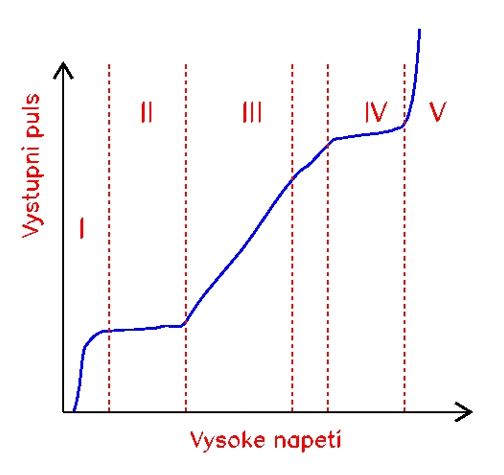
\includegraphics[width=0.6\textwidth]{JS3_plyn.png}
	\caption{Jednotlivé pracovní oblasti plynových detektorů}		
\end{figure}

\textbf{Polohově citlivé}:
\begin{itemize}
	\item Mnohodrátové proporcionální komory - mezi dvěma katodovými rovinami jsou anodové citlivé dráty (signál z nich se snímá)
	\item Driftové komory - drift náboje z ionizace k anodě, typické driftové rychlosti $\sim 5 ~\mathrm{cm/\mu s}$, z času lze určit polohu
	\item Časově projekční komory - cylindr vyplněný plynem zakončený drátovými komorami, umístěno v homogenním magnetickém poli, umožňuje tří rozměrné měření
\end{itemize}

Široké využití ve vysokoenergetické spektrometrii elektronů a pozitronů. 

\subsection{Kanálkový elektronový zesilovač (channeltron)}	

Využívá se pro energie $0,01 - 30 ~\mathrm{keV}$. Kanálek je vyroben ze skla nebo z keramiky. Povrchová vrstva je polovodičová. Zesílení je $\sim 10^7$. Mají malou citlivost na detekci $\gamma$. Můžeme je seskupit do kanálkových desek - miliony miniaturních elektronových zesilovačů pracujících nezávisle. Zesílení je $\sim 10^4$, pro dvě v kaskádě potom $\sim 10^7$. 

\textbf{Polohově citlivý}: vzdálenost kanálků je $8 - 30 ~\mathrm{\mu m}$. 

Mají malou citlivost na magnetické pole. Mrtvá doba se pohybuje okolo $\sim 10 ~\mathrm{ns}$. 
	
\subsection{Polovodičové detektory}

Intenzivně se využívají křemíkové polovodičové detektory. Energetické rozlišení se pohybuje okolo $\sim 0,9 - 1,9 ~\mathrm{keV}$ pro energie $100 - 1000 ~\mathrm{keV}$. Pro nižší energie je důležité co nejtenčí okénko, aby byla co nejmenší absorpce. Využívá se magnetického transportéru - magnetické pole přepraví elektrony do místa s menším pozadím. 

\textbf{Polohově citlivé detektory}:
\begin{itemize}
	\item Křemíkové stripové detektory - na křemíkové destičce (tloušťky $300 ~\mathrm{\mu m}$) jsou tenké proužky z hliníku ($1 ~\mathrm{\mu m}$) a pod ní je $p^+$ implantace (bor) - fungují jako  separátní elektrody
	\item Křemíkové pixelové detektory - struktura do jednotlivých buněk
	\item Křemíkové driftové detektory - struktura elektrod, náboj pak driftuje v elektrickém poli, jedna ze souřadnic je určena z času driftu
\end{itemize}
	
\subsection{Elektrostatické a magnetické spektrometry}

Nabitá částice se pohybuje v magnetickém a elektrickém poli:
\begin{itemize}
	\item elektrické pole - působí síla: $\overrightarrow{F_e} = e \cdotp \overrightarrow{E}$
	\item magnetické pole - působí síla: $\overrightarrow{F_M} = e \cdotp v \times \overrightarrow{B}$
\end{itemize}

Je-li $\overrightarrow{B} \bot \overrightarrow{v}$, potom platí $F = ma = m \dfrac{v^2}{r} = e v B$ a tedy $p = mv = eBr \Rightarrow \dfrac{\Delta p}{p} = \dfrac{\Delta (Br)}{Br}$, kde $m$ je relativistická hmotnost elektronu: $m = \dfrac{m_e}{\sqrt{1 - \left( \dfrac{v}{c}\right)^2 }}$.

Rozlišení magnetických spektrometrů dáno rozlišením hybností:
\begin{equation}
R = \dfrac{\Delta p}{p} = \dfrac{\Delta (Br)}{Br}, ~~~~~~~ FWHM = \Delta (Br)
\end{equation}

Rozlišení elektrostatických spektrometrů dáno rozlišením energie: $R = \dfrac{\Delta E_{KIN}}{E_{KIN}}, ~ FWHM = \Delta E_{KIN}$

Určíme vztah $E_{KIN} = f(Br)$ ($mc^2 - m_e c^2$):
\begin{equation}
m = \dfrac{m_e}{\sqrt{1 - \dfrac{v^2}{c^2}}} \Rightarrow m^2 c^2 \left( 1 - \dfrac{v^2}{c^2}\right) = m_{e}^2 c^2 \Rightarrow m^2 c^2 - m^2 v^2 = m_{e}^2 c^2 \Rightarrow m^2 c^2 - (e B r)^2 = m_{e}^2 c^2
\end{equation}
\begin{equation}
mc^2 = m_e c^2 + E_{KIN} = \sqrt{(m_e c^2)^2 + e^2 (Br)^2c^2} \Rightarrow E_{KIN} = m_e c^2 \left[ \sqrt{1 + \left( \dfrac{e}{m_e c}\right)^2 \cdotp (Br)^2 } - 1\right] 
\end{equation}

\textbf{Určíme vztah mezi rozlišením energetickým a rozlišením hybnostním}:
\begin{equation}
E_{KIN} = \sqrt{p^2 c^2 + m_{e}^2 c^4 } - m_e c^2 \Rightarrow dE_{KIN} = \dfrac{pc^2}{\sqrt{p^2 c^2 + m_{e}^2 c^4}}dp
\end{equation}
a tedy:
\begin{equation}
\dfrac{dE_{KIN}}{E_{KIN}} = \dfrac{p^2 c^2}{ E_{KIN} \sqrt{p^2 c^2 + m_{e}^2 c^4}} \dfrac{dp}{p} = \dfrac{E_{KIN}^2 + 2 E_{KIN} m_e c^2}{E_{KIN} (E_{KIN} + m_e c^2)} \dfrac{dp}{p} = \left( 1 + \dfrac{m_e c^2}{E_{KIN} + m_e c^2}\right) \dfrac{dp}{p} 
\end{equation}
hledaný vztah mezi rozlišeními: 
\begin{equation}
\dfrac{dp}{p} = \dfrac{d(Br)}{Br} \Rightarrow \dfrac{dE_{KIN}}{E_{KIN}}= \left( 1 + \dfrac{m_e c^2}{E_{KIN} m_e c^2}\right) \dfrac{d(Br)}{Br}
\end{equation}

V nerelativistickém případě:
\begin{equation}
E_{KIN} = \dfrac{p^2}{2 m_e} \Rightarrow dE_{KIN} = \dfrac{2p}{2 m_e} dp = \dfrac{p}{m_e} dp
\end{equation}
\begin{equation}
\dfrac{dE_{KIN}}{E_{KIN}} = \dfrac{1}{E_{KIN}} \dfrac{p^2}{m_e} \dfrac{dp}{p} = 2 \dfrac{dp}{p},
\end{equation}
což souhlasí s nerelativistickou limitou( $E_{KIN} << m_e c^2$).

V ultrarelativistickém případě:
\begin{equation}
E_{KIN} = E = pc \Rightarrow \dfrac{dE_{KIN}}{E_{KIN}} = \dfrac{dp}{p},
\end{equation}
což souhlasí s ultrarelativistickou limitou ($E_{kIN} >> m_e c^2$).

\subsection{Základní charakteristiky elektronových spektrometrů}

\begin{itemize}
	\item rozsah měřených energií: $0,01 - 1000 ~\mathrm{keV}$
	\item už zmíněné rozlišení $R\sim 8 \cdotp 10^{-8} - 10^{-1}$
	\item prostorový úhel do kterého letí detekované elektrony $\Omega$: $0,0001 - 20 \%$ ze $4 \pi$
	\item rozměr zdroje nebo ozařovaného terče $\sigma\sim 0,5 ~\mathrm{mm^2} - 200 ~\mathrm{cm^2}$
	\item transmise $T$: část z monoenergetického svazku elektronů, které projdou do detektoru
	\item celková luminosita $L = T \cdotp \sigma\sim 10^{-7} - 10^{-1} ~\mathrm{cm^2}$
	\item Elektron-optická kvalita: $T/R$ nebo $L/R$
	\item intenzita používaných magnetických polí $B\sim 0,0001 - 3 ~\mathrm{T}$
\end{itemize}

Velmi důležitá příprava zdroje - vyloučení energetických ztrát elektronů v materiálu zdroje.

\subsection{Elektrostatické spektrometry}

Používají se do energie $50 ~\mathrm{keV}$ (pro vyšší energie je potřeba příliš velké napětí a je problém s relativistickou korekcí). 
\begin{itemize}
	\item magnetické pole - fokusuje elektrony do měřícího místa, s využitím clon se provádí selekce hybností (energií)
	\item elektrické pole - vytváří potenciálovou bariéru, která propustí elektrony, jejichž energie je větší než jistý práh
	\item integrální způsob měření - při každém měření  (daný brzdící potenciál)
	\item diferenciální způsob měření - pohyb v magnetickém poli vymezí jen určitou energetickou oblast
\end{itemize}

Jednokanálový způsob měření $\rightarrow$ velký důraz je kladen na časovou stabilitu a průběžnou kalibraci

Používané detektory:
\begin{itemize}
	\item kanálkový násobič - výhodné pro nízké energie $\sim ~\mathrm{keV}$
	\item mikrokanálková destička je pozičně citlivá
	\item křemíkový detektor - může měřit i energii
	\item driftové a pixelové detektory - pozičně citlivé
\end{itemize}

\subsection{Magnetické spektrometry}

Magnetické pole je využito k určení hybnosti (energie) elektronu. Rozlišení je $R = \Delta p/p = 10^{-3} \div 10^{-2}$. Během posledních let používána řada typů:
\begin{itemize}
	\item rovinné spektrometry - pole má rovinnou symetrii
	\item čočkový typ - pole má osovou symetrii
\end{itemize}

Typ pomeranč, minipomeranč (\quotedblbase orange, miniorange\textquotedblright ~spectrometer) - magnety jsou rozděleny do sektorů, většinou šest sektorů rozmístěných kolem osy.

Jsou to kompaktní zařízení, magnety vytváří homogenní pole - změnami sestavy magnetů se dá měnit energie maxima transmise a tím i účinnost spektrometru.

\begin{center}
	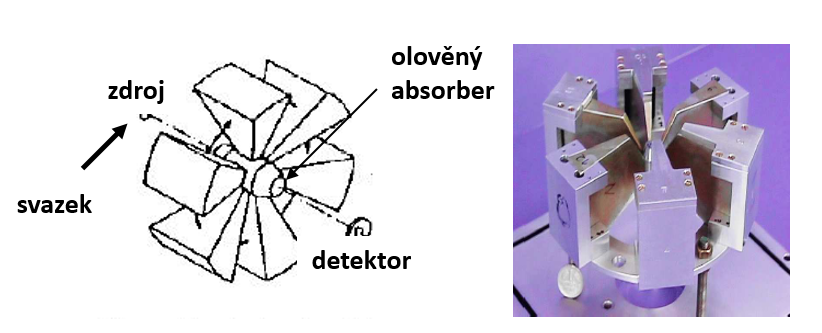
\includegraphics[width=0.8\textwidth]{JS3_minipomeranc.png}
	\captionof{figure}{Spektrometr typu minipomeranč (Universita Bohn)}		
\end{center}

\subsection{Magnetický transportér a křemíkový detektor}

Probíhá měření na svazku $\rightarrow$ vysoké pozadí $\gamma$ fotonů a dalších částic. Magnetické pole je využito pro transport elektronů mimo toto pozadí, energie elektronů je potom určena křemíkovým detektorem. Existuje \quotedblbase jemný přechod\textquotedblright ~mezi magnetickými spektrometry a transportéry. 

Využití:
\begin{itemize}
	\item toroidního magnetického pole: pohyb po cykloidě
	\item magnetického pole solenoidu: $B_z = B, B_x = B_y = 0 \rightarrow $ pohyb po spirále
\end{itemize}	

Činnost systému je dána transmisí transportního systému i účinností detektoru. Některé spektrometry typu pomeranč a minipomeranč mohou být využívány jako trasportéry.
\subsection{Vysokoenergetická fyzika - dileptonové spektrometry}

Používají se ke zkoumání rozpadu částic do $e^+ e^- $ nebo $\mu^+ \mu^- $ kanálu, produkce těchto párů přes virtuální foton $\rightarrow$ nutnost spektrometru leptonů s vysokou energií.

Složení spektrometru:
\begin{itemize}
	\item nutné pro určení hybnosti a odlišení kladných a záporných částic
	\begin{itemize}
		\item velmi intenzivní magnet (často supravodivý)
		\item polohově citlivé detektory před a za magnetem (mnohodrátové proporcionální komory, Čerenkovovy detektory)
	\end{itemize}
	\item vylepšující identifikaci částic (potlačení hadronového pozadí)
	\begin{itemize}
		\item detektory odlišující hadronové a elektromagnetické spršky
		\item detektory měřící dobu letu
	\end{itemize}
\end{itemize}

\begin{center}
	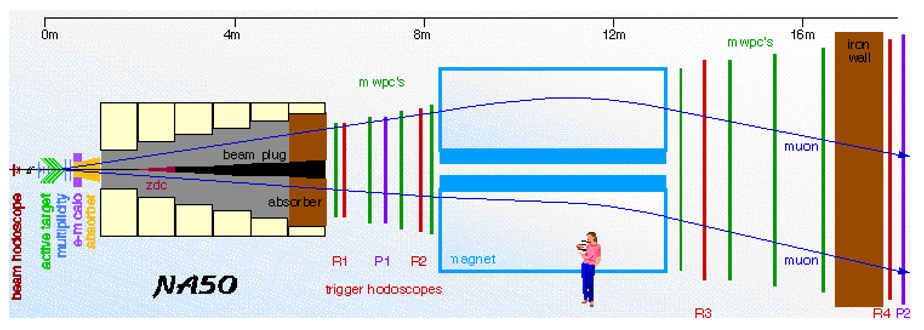
\includegraphics[width=1\textwidth]{JS3_dilepton.png}
	\captionof{figure}{Schéma di-leptonového spektrometru NA50 a jeho dráhové komory}		
\end{center}


\subsection{Použití detektorů Čerenkovova záření}

Čerenkovův detektor je detektor částic, který využívá Čerenkovovo záření vznikající při průchodu částice látkou rychlostí vyšší než je rychlost světla v dané látce. Protože toto záření vytváří charakteristický kužel, lze z jeho vrcholového úhlu $ \vartheta _{c}$ odvodit rychlost částice:
\begin{equation}
\cos \vartheta_c = \dfrac{c}{nv},
\end{equation}
kde $c$ je rychlost světla, $n$ je index lomu v dané látce.

Pokud se z jiného jevu odvodí hybnost takové částice, například z poloměru pohybu částice v magnetickém poli, lze určit i hmotnost sledované částice, což umožňuje její identifikaci.

Tento typ detektorů používají například experimenty CERES a HADES. 

	
\section{Aplikace spektroskopie lehkých nabitých částic}

Uplatnění spektroskopie elektronů:
\begin{itemize}
	\item Studium struktury jader, jaderných přeměn a jaderných reakcí
	\begin{itemize}
		\item studium konverzních elektronů
		\item studium elektronů a pozitronů z rozpadu $\beta$
		\item studium Augerových elektronů
		\item určování hmotnosti elektronových neutrin
		\item studium di-leptonových párů ve vysokoenergetické fyzice	
	\end{itemize}
    \item Aplikace
    \begin{itemize}
    	\item spektroskopie energetických ztrát elektronů s vysokým rozlišením
    	\item měření šířek atomových hladin a energií vazby elektronu
    	\item studium molekulárních vazeb z posunu energie linek konverzních eelktronů
    \end{itemize} 
\end{itemize}

Spektrum elektronů je:
\begin{itemize}
	\item spojité - z rozpadu $\beta$ , brzdné záření, ....
	\item diskrétní - konverzní, Augerovy elektrony
\end{itemize}	 
 
\subsection{Studium konverzních elektronů}

\begin{itemize}
	\item Společně se určí intenzita $\gamma$ a elektronů, což umožní určit multipolaritu přechodu
	\item Přechody $E0$ jsou realizovány pouze prostřednictvím elektronů 
	\item velmi častá jsou měření na svazku v součinnosti s $4 \pi$ detektorovými systémy pro detekci záření $\gamma$
	\item Důležitá je oprava na Dopplerův posuv (rozšíření linky ve spektru)
	\item kinematický posuv je popsán Lorentzovskou transformací: 
	\begin{equation}
	E = \gamma E^* \left[ 1 + \dfrac{p^* c}{E^*} \beta \cos \Theta ^* ,\right]  
	\end{equation}
	kde $^* $ označuje souřadný systém spojený s pohybujícím se jádrem
	\item složené jádro $\rightarrow$ stejná rychlost reakce 
	\item kinematiku určíme detekcí jádra
\end{itemize}

\subsection{Studium elektronů a pozitronů z rozpadu $\beta$}

Měří se Fermi-Kurieho graf:
\begin{equation}
\sqrt{\dfrac{N(E_e)}{F^* (Z, E_e)}} = konst. \cdotp (E_{MAX} - E_e),
\end{equation}
kde $N(E_e)$ je počet elektronů, $F^* (Z,E_e)$ je Fermiho funkce, která obsahuje korekci na coulombovské pole jádra i atomového obalu.

Pokud $m_{\nu} c^2 \neq 0 \rightarrow E_{MAX} = Q - m_{\nu}c^2$, kde $Q$ je energie rozpadu. Vždy se určuje kvadrát hmotnosti neutrina. Je zapotřebí velmi vysokého rozlišení a minimalizace možnosti energetických ztrát (narušení tvaru spektra).

\begin{center}
	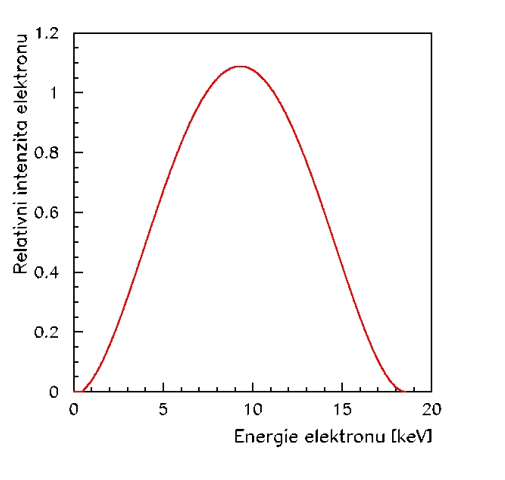
\includegraphics[width=0.6\textwidth]{JS3_neutrino1.png}
	\captionof{figure}{Schematický průběh závislosti $N_e = f(E_e)$ v rozpadu $\beta$}		
\end{center}

\begin{center}
	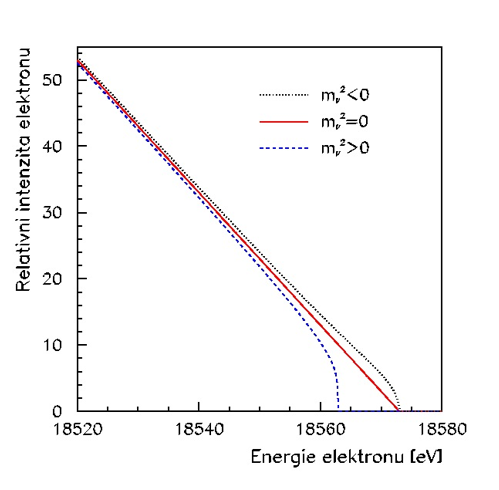
\includegraphics[width=0.6\textwidth]{JS3_neutrino2.png}
	\captionof{figure}{Fermiho graf pro rozpad tritia $^{3}H$, které se nejčastěji využívá k určování hmotnosti neutrina}		
\end{center}

\subsection{Určování hmotnosti neutrin}

Současná hranice pro hmotnost neutrin (experimenty v Mainzu a Troicku) je $m_{\nu} < 2 - 3 ~\mathrm{eV}$. Byla určena záporná hodnota kvadrátu hmotnosti.

Komplikace:
\begin{itemize}
	\item energetické ztráty v terči, molekule $T_2$ 
	\item stabilita přístroje
\end{itemize}	 

Hmotnost neutrina se snaží najít na experimentu KATRIN. Je to integrální elektrostatický spektrometr, který je na Obr. \ref{js3:obr:JS3_katrin}.

\begin{figure}[h]
	\centering
	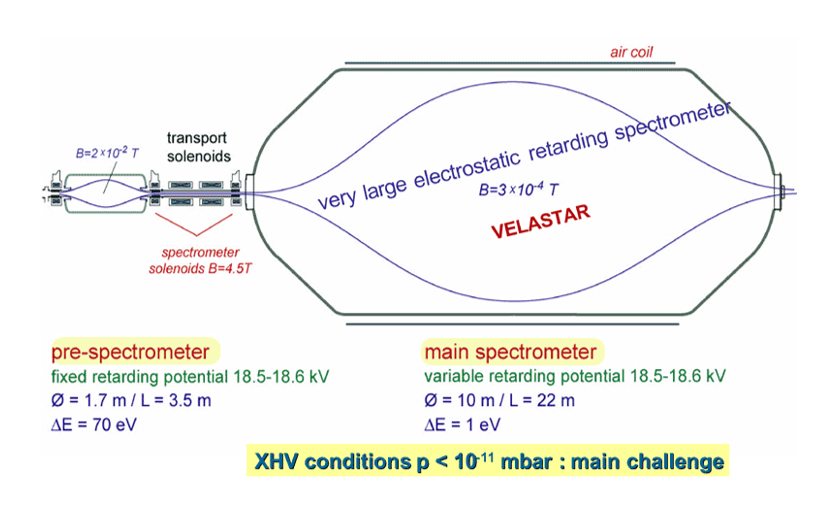
\includegraphics[width=0.9\textwidth]{JS3_katrin.png}
	\caption{Schéma spektrometru KATRIN \label{js3:obr:JS3_katrin}}		
\end{figure}

\begin{figure}[h]
	\centering
	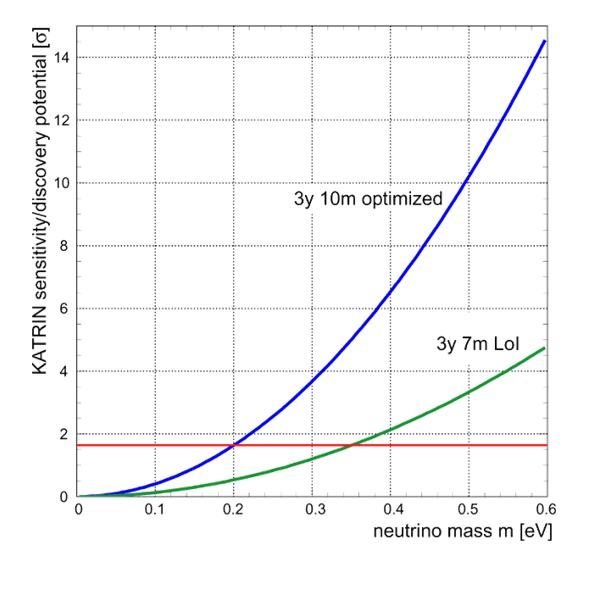
\includegraphics[width=0.5\textwidth]{JS3_katrin2.png}
	\caption{Předpokládaná citlivost spektrometru KATRIN}		
\end{figure}

\subsection{Využití párových spektrometrů pro hledání rozpadů exotických částic}

Některé hypotetické částice by se měly rozpadat na pár elektron - pozitron. Vznikat by mohly například při srážkách těžkých iontů. Na Obr. \ref{js3:obr:JS3_axion} je párový spektrometr APEX, který původně nebyl určen pro hledání axionů. Axiony jsou hypotetické elementární částice, které předpověděli Roberto Peccei a Helen Quinnová v roce 1977. Tyto částice by měly vyřešit problémy CP symetrie v kvantové chromodynamice (QCD) a jsou to hlavně částice, ze kterých by se měla skládat temná hmota.

\begin{center}
	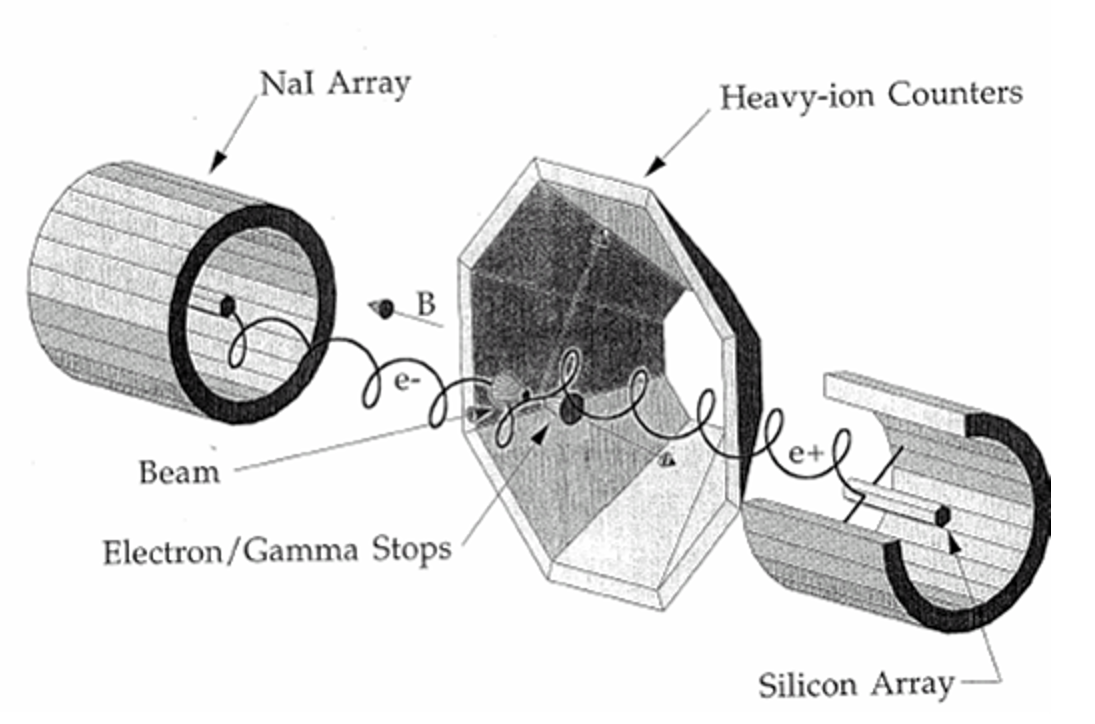
\includegraphics[width=0.8\textwidth]{JS3_axion.png}
	\captionof{figure}{párový spektrometr APEX, který původně nebyl určen pro hledání axionů. Nachází se v Argonne National Laboratory \label{js3:obr:JS3_axion}}		
\end{center}

\subsection{Studium di-leptonových párů ve vysokoenergetické fyzice}

Používají se dráhové spektrometry: CERES, NA50, HADES, ... Důležité je hybnostní rozlišení. A je velmi důležité popsání kombinatorického pozadí. Zdroje párů $e^+ e^- $ jsou na Obr. \ref{js3:obr:JS3_dilepton1}. 

\begin{figure}
	\centering
	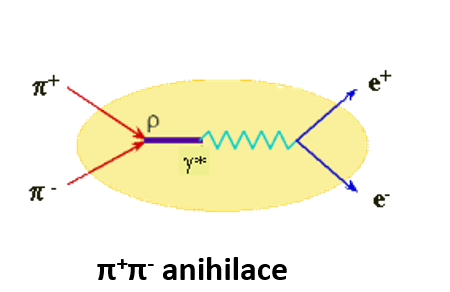
\includegraphics[width=0.4\textwidth]{JS3_dilepton1.png}
	\caption{Zdroje párů $e^+ e^-$ \label{js3:obr:JS3_dilepton1}}		
\end{figure}
\begin{figure}
	\centering
	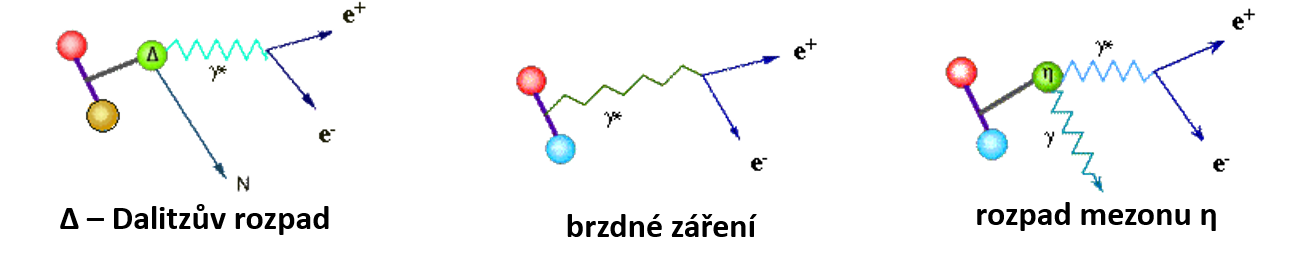
\includegraphics[width=1\textwidth]{JS3_dilepton2.png}
	\caption{Zdroje párů $e^+ e^-$ \label{js3:obr:JS3_dilepton2}}		
\end{figure}
\begin{figure}
	\centering
	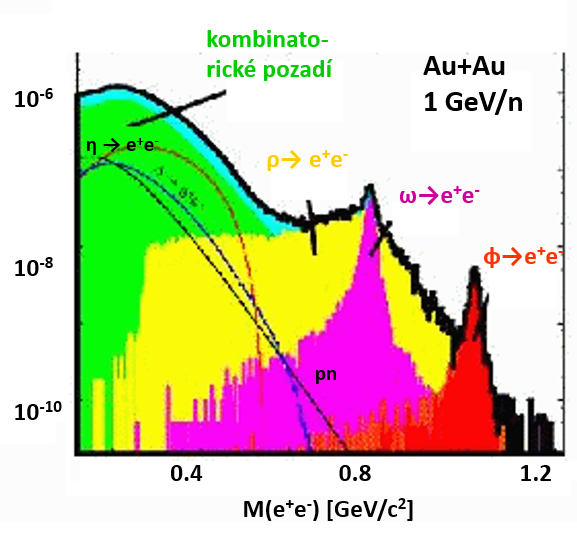
\includegraphics[width=0.6\textwidth]{JS3_dilepton3.png}
	\caption{Dileptonový "koktejl"\label{js3:obr:JS3_dilepton3}}		
\end{figure}

\subsection{Spektroskopie energetických ztrát elektronů s vysokým rozlišením}

sestava:
\begin{itemize}
	\item elektronové dělo - elektrony
	\item elektronový spektrometr s vysokým rozlišením
\end{itemize}
Využití:
\begin{itemize}
	\item zkoumání povrchů pomocí charakteristických Augerových elektronů, rozptylu elektronů, elektronové difrakce
	\item studium struktury
\end{itemize}

\textbf{XPS metoda} je rentgenová fotoelektronová spektroskopie - povrchová, chemická analýza. Základem je proces fotoelektronové a sekundární elektronové emise. Spektrometry mají dvě základní součásti – primární zdroj a elektronový analyzátor. Ze samotného principu vyplývá, že musí pracovat v podmínkách nízkých tlaků (nezbytných pro provoz žhavých katod a elektronových násobičů) zajišťujících dostatečně dlouhé střední volné dráhy elektronů pro jejich pohyb v systému vzorek – detektor. Ve skutečnosti jsou spektrometry provozovány při velmi nízkých tlacích (v podmínkách ultra-vysokého vakua), kde výše zmíněné důvody nejsou zdaleka limitujícím faktorem. UHV podmínky jsou nezbytné pro přípravu čistých povrchů analyzovaných vzorků s vyloučením vlivu adsorpce plynů, a pro udržení takto čistých povrchů po dobu měření (poznamenejme zde, že teprve při tlaku v oblasti od  10-7 Pa je možno počítat dobu vytvoření jedné povrchové monovrstvy v desítkách minut). A právě nutnost ultravysokovakuového provedení je jedním z faktorů vysoké technologické a tudíž i cenové náročnosti těchto metod. 

\end{document}